\documentclass[letter]{article}
\usepackage[spanish]{babel}
\usepackage[margin=1in]{geometry}
\usepackage{amsmath}
\usepackage{amsthm}
\usepackage{amssymb}
\usepackage[utf8]{inputenc}
\usepackage{graphicx, color}
\usepackage{algorithm}
\usepackage{algpseudocode}
\usepackage{mathrsfs}


% Some definitions
\floatname{algorithm}{Algoritmo}

% Author info
\title {Secuencia más larga de vecinos que están ordenados}
\author{ Jorge Luis Esposito Albornoz$^1$  Juan Sebastián Herrera Guaitero$^1$}
\date{
	$^1$Departamento de Ingeniería de Sistemas, Pontificia Universidad Javeriana\\Bogotá,  Colombia \\
	\texttt{\{jesposito,jsebastianherrera\}@javeriana.edu.co}\\~\\
	\today
}

\begin{document}
\maketitle

\begin{abstract}
	En este documento se presenta la formalización del problema de encontrar la secuencia más larga de vecinos que están ordenados.
	\textbf{Palabras clave:} matriz, adyacentes.
\end{abstract}

\tableofcontents

\newpage
\section{Formalización problema}
El problema de encontrar la secuencia mas larga de vecinos que estan ordenados, es un problema muy utilizado en el mundo empresarial para realizar entrevistas de conocimiento
a los candidatos. Su dificultad particular radica en la soluc\'ion del problema, los primeros acercamientos a la soluc\'ion suelen ser a trav\'es
de la recursi\'on ingenua, sin embargo, utilizar programaci\'on din\'amica es una buena opci\'on.

\subsection{Definición del problema}
Dada una matriz cuadrada natural de tamaño $NxN$, que contiene los números únicos en el rango $[1,NxN]$, pero que no están forzosamente en orden, encontrar la secuencia más larga de vecinos que están ordenados y los elementos adyacentes en la matriz que tienen una diferencia de $+1$.
\break
\break
El problema de la secuencia mas larga de vecinos ordenados se define apartir de:
\begin{enumerate}
	\item Una matriz $M$ de elementos $a\in\mathbb{Z}$.
\end{enumerate}
Generar una secuencia $S$ cuyos elementos cumplan con una relac\'ion $a<b$.
\begin{itemize}
	\item \textbf{Entradas:}
	      \begin{itemize}
		      \item $M^{nxn} ~ | ~ \forall M_{ij} \in \mathbb{Z} \right>\right>$
	      \end{itemize}
	\item \textbf{Salidas:}
	      \begin{itemize}
		      \item $S = \left<s_i \in M\right> ~ | ~ \forall i \in M ~ s_i \le s_{i+1}  $
	      \end{itemize}
\end{itemize}
\section{Algoritmo de soluci\'on}
\subsection{Idea soluci\'on}
\begin{figure}[H]
	\centerline{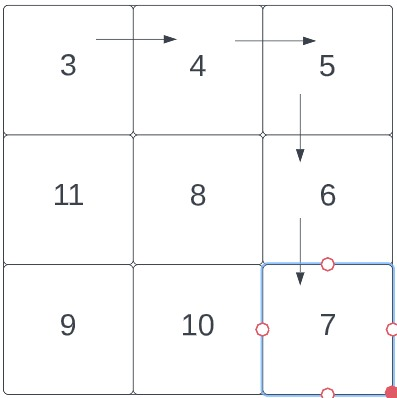
\includegraphics[scale=0.30]{sample.jpg}}
	\caption{Matriz inicial}
	\label{fig}
\end{figure}
Se planteo la siguiente ecuaci\'on como posible soluci\'on del problema: \\
\[ M_{ij} =
	\begin{cases}
		\quad 0 & \text{if } |M| = 0 \\
		\quad \[ max=
			\begin{cases}
				M_{i-1j} & \quad \text{if } ~ i  >  1 ~ \land ~ M_{ij}+1 = M_{i-1j}   \\
				M_{i+1j} & \quad \text{if } ~ i  <  |M| ~ \land ~ M_{ij}+1 = M_{i+1j} \\
				M_{ij-1} & \quad \text{if } ~ j  >  1 ~ \land ~ M_{ij}+1 = M_{ij-1}   \\
				M_{ij+1} & \quad \text{if } ~ j  <  |M| ~ \land ~ M_{ij}+1 = M_{ij+1} \\
			\end{cases}
		\]
	\end{cases}
\]
Teniendo en cuenta que para cada posici\'on $ij$ dentro de la matriz pueden existir valores
adyacentes se busca obtener el valor m\'aximo.

\subsection{Escritura del algor\'itmo}
\begin{algorithm}[!htb]
	\caption{Max num}
	\begin{algorithmic}[1]
		\Function{$max$}{$a,b$}
		\If{$a > b$}
		\State \Return $a$
		\Else
		\State \Return $b$
		\EndIf
		\EndFunction
	\end{algorithmic}
\end{algorithm}
\begin{algorithm}[!htb]
	\caption{aux}
	\begin{algorithmic}[1]
		\Procedure{$max$}{$T,M,B,i,j$}
		\State $q \gets 0$
		\If{$|T| = 0$}
		\State \Return $0$
		\If{$M_{ij} \neq 0$}
		\State \Return $M_{ij}$
		\Else
		\If{$i > 0 ~ \land ~ T_{ij}+1 = T_{i-1j}$}
		\State $q \gets \Call{max}{q,AUX(T,M,B,i-1,j)}$
		\If{$ q = M_{i-1j}$}
		\State $B_{ij} \gets pair(i-1,j)$ \Comment Pair pareja de elementos
		\EndIf
		\EndIf
		\If{$i < |T| ~ \land ~ T_{ij}+1 = T_{i+1j}$}
		\State $q \gets \Call{max}{q,AUX(T,M,B,i+1,j)}$
		\If{$ q = M_{i-1j}$}
		\State $B_{ij} \gets pair(i+1,j)$ \Comment Pair pareja de elementos
		\EndIf
		\EndIf
		\If{$j > 0 ~ \land ~ T_{ij}+1 = T_{ij-1}$}
		\State $q \gets \Call{max}{q,AUX(T,M,B,i,j-1)}$
		\If{$ q = M_{ij-1}$}
		\State $B_{ij} \gets pair(i,j-1)$ \Comment Pair pareja de elementos
		\EndIf
		\EndIf
		\If{$j < |T| ~ \land ~ T_{ij}+1 = T_{ij+1}$}
		\State $q \gets \Call{max}{q,AUX(T,M,B,i,j+1)}$
		\If{$ q = M_{ij+1}$}
		\State $B_{ij} \gets pair(i,j+1)$ \Comment Pair pareja de elementos
		\EndIf
		\EndIf
		\State $M_{ij} \gets q + 1 $
		\EndIf
		\State \Return $M_{ij}$
		\EndProcedure
	\end{algorithmic}
\end{algorithm}
\begin{algorithm}
	\caption{LSNBacktracking}
	\begin{algorithmic}[1]
		\Procedure{$bactraking$}{$T$}
		\State \textbf{let }$M$ \textbf{ be a matrix filled with } $0$
		\State \textbf{let }$B$ \textbf{ be a matrix filled with pairs of integers}
		\State \textbf{let }$rt$ \textbf{ be an array}
		\State \textbf{let }$current$ \textbf{ be a pair of integers}
		\State $q \gets 0$
		\For{ $i \gets 1 ~ \textbf{to} ~ |T|$ }
		\For{ $j \gets 1 ~ \textbf{to} ~ |T|$ }
		\State $q \gets \Call{max}{q,AUX(T,M,B,i,j)}$
		\If{$q = M_{ij}$}
		\State $\textbf{let }current \textbf{ be a pair that stored i and j}$
		\EndIf
		\EndFor
		\EndFor
		\While{$B_{current_{1}current_{2}} ~ \neq ~ current $}
		\State \textbf{let } $rt$ \textbf{ add  } $T_{current_1current_2}$
		\State $current \gets B_{current_1current_2}$
		\EndWhile
		\State \textbf{let } $rt$ \textbf{ add  } $T_{current_1current_2}$
		\State \Return rt
		\EndProcedure
	\end{algorithmic}
\end{algorithm}
\textbf{An\'alisis de complejidad:}
O(N*N)\\
\textbf{Invariante:}La tabla se esta llenando correctamente.


\section{An\'alisis experimental}
En esta secci\'on encontrar\'a el an\'alisis experimental del problema de la secuencia mas larga de vecinos adyacentes con una diferencia de $+1$ en una matriz $NxN$.
\subsection{Protocolo}
\begin{enumerate}
	\item Elegir uno de los archivos de la carpeta input para probar en el programa.
	\item Pasar como par\'ametro de lanzamiento la ruta del archivo elegio.
	\item Correr el algoritmo para obtener la secuencia m\'as larga de vecinos ordenados.
\end{enumerate}
\subsection{Matrices definidas}
\subsubsection{Procedimiento}
\begin{enumerate}
	\item Se eligi\'o como archivo de entrada el archivo input/test.csv que contiene el ejemplo dado en el enunciado.
	\item Se procedi\'o a compilar el archivo main.cpp de la siguiente manera: $$g++ ~ main.cpp -o ~ main ~ \&\& ~ ./main ~ ruta\_archivo.$$
	\item Se obtuvo como resultado $2,3,4,5,6,7,8,9,10$.
\end{enumerate}
\newpage
\subsubsection{Resultado}
\begin{enumerate}
	\item  \textbf{Entrada:} test.csv\\
	      \begin{figure}[H]
		      \centering
		      \begin{matrix}
			      4,  & 4   &     &    \\
			      10, & 16, & 15, & 12 \\
			      9,  & 8,  & 7,  & 13 \\
			      2,  & 5,  & 6,  & 14 \\
			      3,  & 4,  & 1,  & 11 \\
		      \end{matrix}
	      \end{figure}
	\item Al leer el archivo la matriz queda guardada de la siguiente manera:\\
	      \begin{figure}[H]
		      \centering
		      \begin{pmatrix}
			      10 & 16 & 15 & 12 \\
			      9  & 8  & 7  & 13 \\
			      2  & 5  & 6  & 14 \\
			      3  & 4  & 1  & 11 \\
		      \end{pmatrix}
	      \end{figure}
	\item \textbf{Resultado esperado:} $2,3,4,5,6,7,8,9,10$.
	\item \textbf{Resultado obtenido:} $2,3,4,5,6,7,8,9,10$.


\end{enumerate}
\subsection{Matrices aleatorias}
\subsubsection{Procedimiento}
\begin{enumerate}
	\item Ejecutar script de python de la siguiente manera:$$py ~~ create\_files.py ~~ n >> nombre\_archivo$$\\
	      \textbf{n representa cualquiera n\'umero entero.}
	\item Elegir el archivo de entrada generado por el script de python.
	\item Se procedi\'o a compilar el archivo main.cpp de la siguiente manera: $$g++ ~ main.cpp -o ~ main ~ \&\& ~ ./main ~ ruta\_archivo.$$
	\item Se obtuvo como resultado $3,4$.
\end{enumerate}
\subsubsection{Resultado}
\begin{enumerate}
	\item  \textbf{Entrada:} random5.csv\\
	      \begin{figure}[H]
		      \centering
		      \begin{matrix}
			      5,  & 5   &     &     &    \\
			      19, & 17, & 1,  & 2,  & 14 \\
			      11, & 23, & 15, & 5,  & 12 \\
			      13, & 7,  & 21, & 9,  & 20 \\
			      25, & 10, & 4,  & 18, & 6  \\
			      16, & 8,  & 3,  & 22, & 24
		      \end{matrix}
	      \end{figure}
	\item Al leer el archivo la matriz queda guardada de la siguiente manera:\\
	      \begin{figure}[H]
		      \centering
		      \begin{pmatrix}
			      19 & 17 & 1  & 2  & 14 \\
			      11 & 23 & 15 & 5  & 12 \\
			      13 & 7  & 21 & 9  & 20 \\
			      25 & 10 & 4  & 18 & 6  \\
			      16 & 8  & 3  & 22 & 24
		      \end{pmatrix}
	      \end{figure}
	\item \textbf{Resultado esperado:} $3,4$.
	\item \textbf{Resultado obtenido:} $3,4$.


\end{enumerate}

\subsection{An\'alisis}
Durante el camino a la soluci\'on logramos deducir que la complejidad temporal es  $O(n*n)$, donde n es el número de filas y de columnas para nuestra caso en particular sabiendo que estamos trabajando con matrices cuadradas. Esto se debe a que estamos calculando los valores de todas las celdas una vez y hay un total de $n*n$ celdas.

De igual modo, la complejidad espacial es $O(n*n)$, puesto que estamos almacenando los valores de todas las celdas, lo que ocupará un espacio $O(n*n)$ y la propia matriz ocupará otro espacio $O(n*n)$. Por tanto, la complejidad espacial total es $O(2(n*n))$, pero omitiendo las constantes tenemos  $O(n*n)$.

\end{document}

